\documentclass[conference]{IEEEtran}
\usepackage{cite}
\usepackage{array}
\usepackage{url}
\usepackage{graphicx}
\usepackage{todonotes}
\usepackage{hyperref}

% correct bad hyphenation here
\hyphenation{op-tical net-works semi-conduc-tor}


\begin{document}

\title{ArKanjo: a tool for detecting function-level Code Duplication in the Linux Kernel}


% author names and affiliations
% use a multiple column layout for up to three different
% affiliations
\author{\IEEEauthorblockN{Luan Arcanjo}
\IEEEauthorblockA{
Universidade de São Paulo, Brazil\\
luanicaro@usp.br}
\and
\IEEEauthorblockN{David Tadokoro}
\IEEEauthorblockA{
Universidade de São Paulo, Brazil\\
davidbtadokoro@usp.br}
\and
\IEEEauthorblockN{Paulo Meirelles}
\IEEEauthorblockA{
Universidade de São Paulo, Brazil\\
paulormm@ime.usp.br}

}

% make the title area
\maketitle

% As a general rule, do not put math, special symbols or citations
% in the abstract
\begin{abstract}
The Linux kernel massive scale (+28 M LoC, +20 K contributors) presents unique 
maintenance challenges. Surprisingly, code duplication remains a persistent issue 
in the kernel codebase, which can hinder its evolution and patching. Academic 
approaches often focus on pairwise comparison of code artifacts, which are not directly applied 
to comprehensive codebase analyses. Other existing free
software\footnote{In this paper, we use the term \textit{Free Software}
interchangeably with \textit{Open Source Software}.} tools explored in 
practice frequently suffer from limited functionality, such as primitive textual 
matching, prove too narrow in scope, or fail to deliver effective results on complex, 
large-scale codebases. Existing solutions generally fail to address the Linux kernel 
specific needs: (1) scalability to handle its size, (2) actionable results for 
developers, and (3) integration with kernel development workflows.
%
This paper presents \textit{ArKanjo}, a novel command-line tool for Linux kernel maintenance 
designed to detect and analyze function-level duplications. Released under the MIT 
license, ArKanjo employs a two-stage architecture consisting of a Preprocessor and 
a Query Responder that separates computationally intensive analysis from efficient 
querying for duplications within large codebases. Pivotal advantages of ArKanjo over 
existing solutions include: (1) preprocessing that enables rapid queries without redundant analysis; 
and (2) prioritization of duplicates that impact maintainability, such as copied 
buggy logic. 
%
We evaluate ArKanjo against real-world duplication cases in recent 
kernel versions, demonstrating its effectiveness in identifying problematic clones 
that generic tools often overlook. By identifying well-defined, manageable 
duplication instances, ArKanjo effectively lowers the barrier for new contributors, 
a capability evidenced by its role in guiding students to make their first code 
improvements to the kernel. ArKanjo offers immediate value to kernel maintainers 
and serves as a replicable model for clone detection in other large-scale free 
software projects.

\end{abstract}

% no keywords

\IEEEpeerreviewmaketitle



\section{Introduction}

The Linux kernel is a foundational free software project 
critical to a significant portion of the world digital infrastructure. Maintaining 
the kernel is an enormous undertaking involving over 28 million lines of code 
and contributions from over twenty thousand developers. Within this context, code 
duplication persists as a significant challenge, a known harmful practice that 
negatively affects code readability and increases the likelihood of introducing
bugs~\cite{harmone,harmtwo}. This issue is particularly acute in the 
kernel device drivers, which comprise over 66\% of the source code~\cite{marcelo}. 
For instance, maintainers of the AMD Display driver have specifically highlighted code 
duplication as a significant impediment to their work.

The detection of code duplication, or code clones, has been a research subject for 
decades~\cite{firstman}. The literature provides a standard taxonomy, classifying 
clones into four types based on their degree of similarity, from identical copies 
(Type-1) to semantically equivalent but textually different fragments (Type-4)~\cite{litreview}. 
Various detection methodologies have been developed, including textual, token-based, 
tree-based, and graph-based approaches~\cite{litreview}. These have culminated in 
state-of-the-art techniques, such as the graph-based work by Liu et al.~\cite{tailor}.

However, the primary focus of such academic work remains on determining whether a given 
pair of code artifacts are duplicates rather than providing a scalable method to scan 
an entire codebase for actionable results. Conversely, existing free software tools explored 
in practice, often lack this sophistication, relying instead on primitive textual matching 
that is insufficient for the complexity and scale of the kernel.

To fill this gap, this research proposes a new approach embodied in \textit{ArKanjo}, a tool 
designed specifically to identify and facilitate the mitigation of function-level code 
duplications within the Linux kernel. We employ multiple analytical 
methods and ethnographic studies to test it.


\section{ArKanjo Tool}

ArKanjo, our proposed tool, is a Command Line Interface (CLI) application designed to
help developers identify code clone duplication at the function level. Released under the
MIT license, ArKanjo is available at 
\textit{\href{https://github.com/arkanjo-tool/arkanjo}{github.com/arkanjo-tool/arkanjo}}.

\subsection{Architecture}

\begin{figure}[ht]
\centering
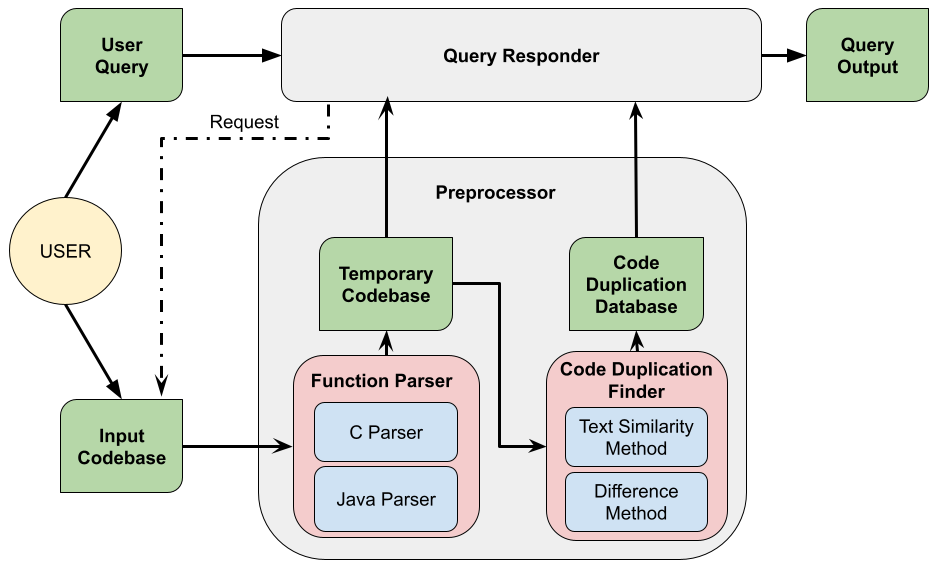
\includegraphics[width=3.5in]{fig/diagrama_mestrado.png}
\caption{Architecture diagram with the tool components}
\label{fig:diagram}
\end{figure}

The tool operates in two main parts, as illustrated in Figure~\ref{fig:diagram}: the \textbf{Preprocessor} and the \textbf{Query Responder}. 
The \textbf{Preprocessor} performs heavy computations to find code 
duplications across a codebase and produces artifacts to store duplication-related information 
in a structured form. The \textbf{Query Responder} consumes the artifacts produced 
by the Preprocessor to execute the tool functionalities as requested. This design allows the 
tool to perform the heavy and time-consuming steps only once per codebase, enabling fast performance 
for multiple queries on the same codebase.

The Preprocessor contains two main components: the Function Breaker and the Code Duplication Finder. 
The workflow of the Preprocessor is as follows: the Function Parser receives the input codebase,
extracts the functions along with metadata, and creates a temporary codebase where each extracted 
function becomes a new code file. The Code Duplication Finder then iterates over every pair of files 
in the temporary codebase, checks whether they are code clones, and, if so, stores the result in 
the Code Duplication Database. This database is a text file that records each code duplication as a triple 
\textbf{$<$function1, function2, similarity$>$}, where \textbf{function1} and \textbf{function2} are the 
duplicated functions, and \textbf{similarity} is the score returned by the duplication detection method 
used in the Code Duplication Finder.

The Query Responder uses the temporary codebase and the Code Duplication Database to extract 
information about duplicated functions based on the user's request. If the user executes the Query Responder
without previously executing the Preprocessor, the Query Responder automatically 
calls the Preprocessor to generate the required artifacts.

The Function Parser receives the input codebase and transforms it into the temporary
codebase. It iterates through every source code file written in a supported programming 
language and uses a language-specific extractor to isolate each function. For each extracted 
function, two new source code files and a metadata file are created in the temporary codebase, 
represented by the pair \textbf{$<$file name, function name$>$}, the source code of the function, 
and the function metadata (in practice, this is a duplication of the original codebase, 
structured as a parsed representation). One of the new files contains the function body, and the other 
contains the function signature. The metadata file includes additional relevant information,
such as the function name, the line where the signature starts, and the line where the function 
body ends. Currently, the supported programming languages are C and Java, although Java support is limited.

The Code Duplication Finder iterates through every pair of source code files in the
temporary codebase, each representing a function from the input codebase. For each pair,
a code duplication detection method computes a similarity score. If the similarity is greater 
than or equal to the minimum threshold (provided by the user during preprocessing), the pair 
is stored in the Code Duplication Database along with the similarity score.

We implemented two duplication detection methods in the tool, which users can choose 
between. The first method is based on text similarity, and the second is a more straightforward approach 
based on the number of identical lines. The experiments and tests in this research were 
conducted using the text similarity method.


\subsubsection{Code Duplication Methods Used}

For the text similarity method, we treat the source code files as plain text and apply the
TF-IDF vector embedding method implemented by the Gensim library~\cite{gensim},
then compute cosine similarity as the similarity metric. We chose this method for 
its reported performance, programming language independence, and the fact that it does 
not require compilable code, an important aspect given that the
temporary codebase does not contain complete code artifacts.

We implemented a more straightforward approach for the difference method,
considering the number of exactly equal lines between two functions.
For two functions, \textit{function1} and \textit{function2}, we compute the similarity as the 
ratio of duplicated lines to the total number of lines across both functions.
This method is considerably simpler and more explainable than the text similarity method, 
The metric is defined by the proportion of common lines between the two functions. 
We use the \textit{diff} command built into the Linux environment to compute the number of equal lines.

\subsection{Functionalities}

We propose three main functionalities for the user in the tool, called Duplication
Explorer, Function Information, and Duplication Report. Each functionality accepts
specific parameters to perform its operations.

\begin{figure}[ht]
\centering
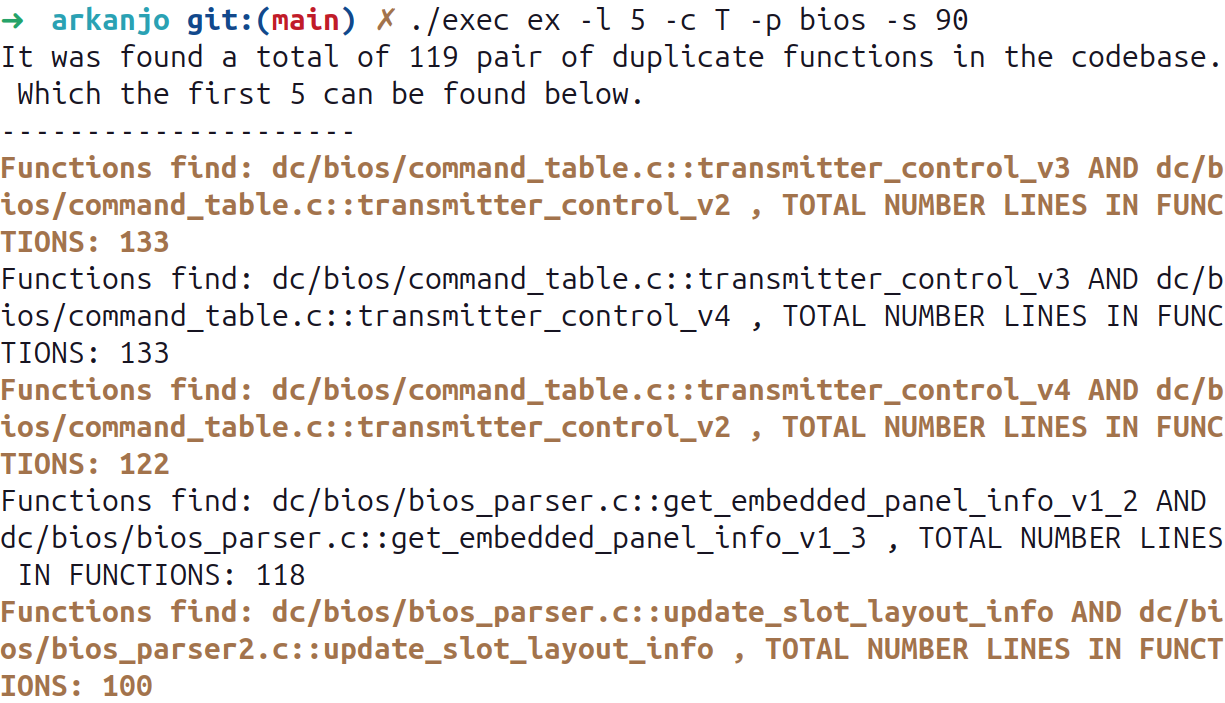
\includegraphics[width=3.5in]{fig/explorer_example.png}
\caption{Example of the \textit{Duplication Explorer} functionality.}
\label{fig:explorer_ex}
\end{figure}

The Duplication Explorer is the primary functionality of our tool, designed to present
the user with pairs of duplicated functions identified by the tool. We implement optional
filters to support more complex queries. Figure~\ref{fig:explorer_ex}
demonstrates an example of this functionality in use.


\begin{figure}[ht]
\centering
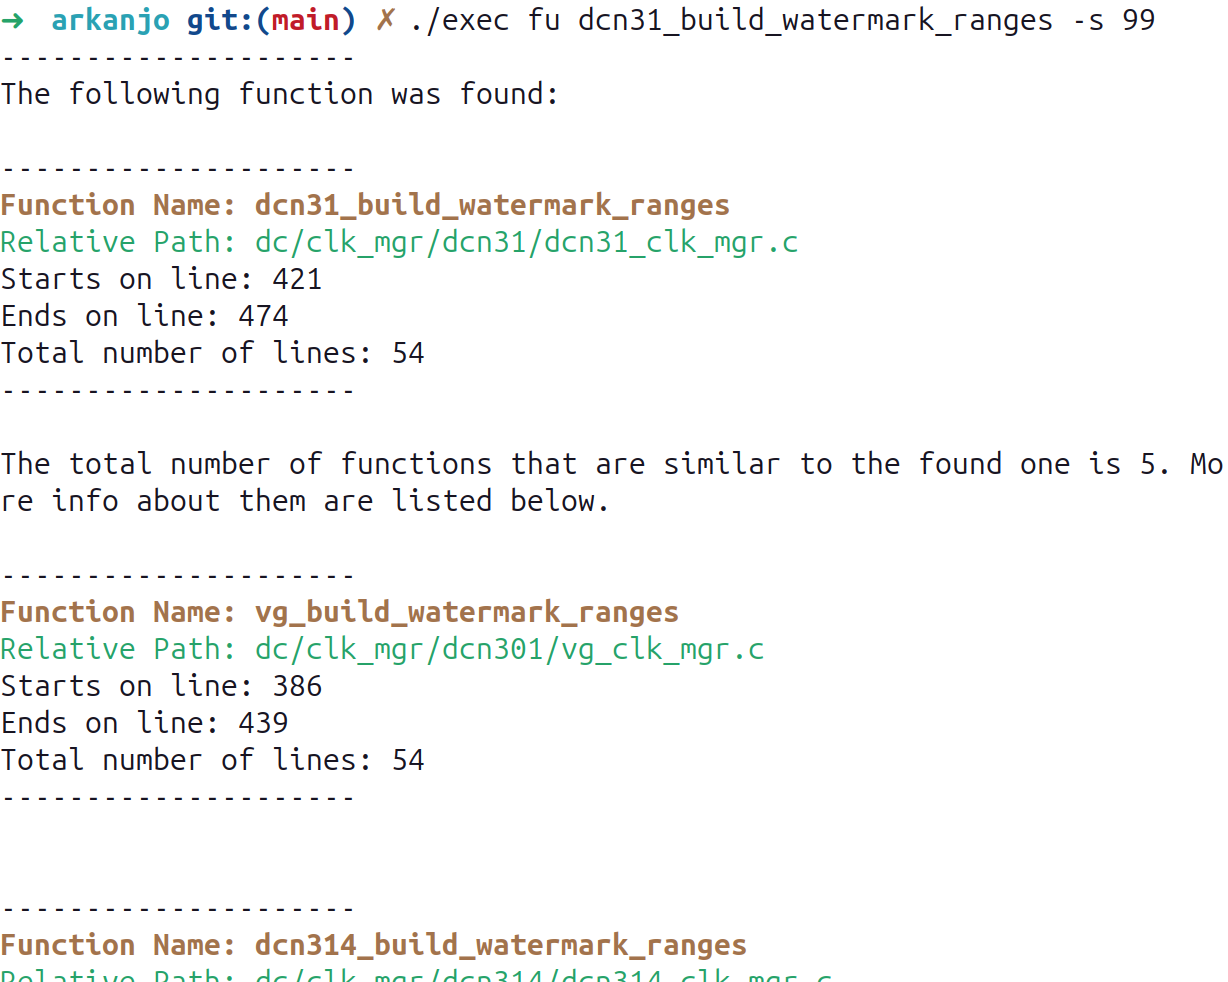
\includegraphics[width=3.5in]{fig/function_example.png}
\caption{Example of the \textit{Function Information} functionality.}
\label{fig:function_ex}
\end{figure}


The Function Information functionality provides detailed information about a specific function. 
It receives a target function from the user
and returns information such as the relative path, function name, and line numbers where
the function is defined. Additionally, it provides similar information for every function
that duplicates the given function. Figure~\ref{fig:function_ex} demonstrates an
example of this functionality in use.

\begin{figure}[ht]
\centering
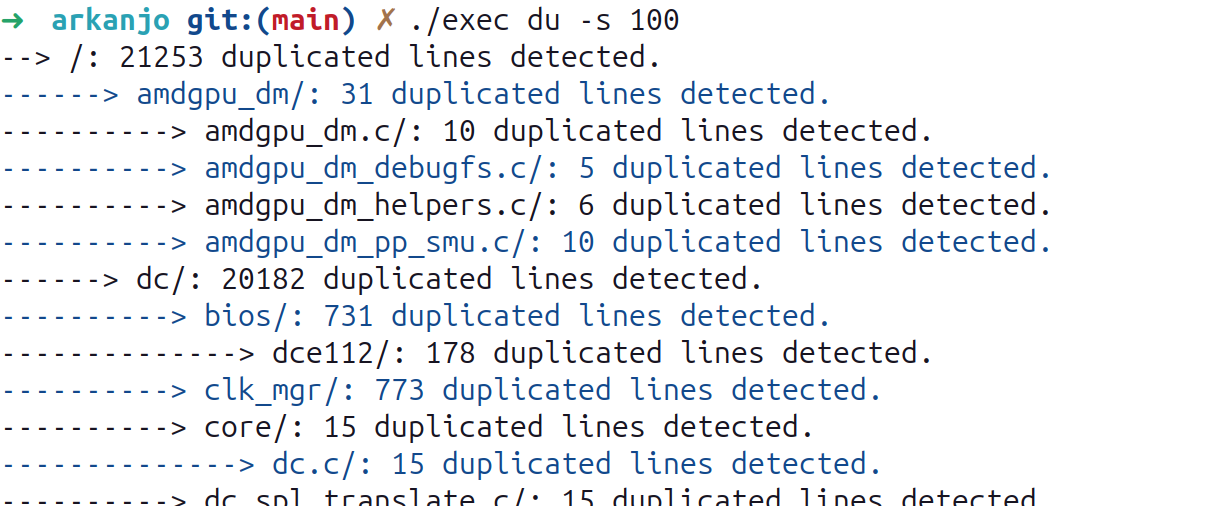
\includegraphics[width=4in]{fig/relatory_example.png}
\caption{Example of the \textit{Duplication Report} functionality.}
\label{fig:relatory_ex}
\end{figure}

The Duplication Report functionality provides an overview of
duplicated code within the input codebase. It calculates the number of
duplicated lines per folder in the codebase and presents the information to the user in
a readable format, as demonstrated in Figure~\ref{fig:relatory_ex}.


\section{Methods}

We applied two independent evaluation approaches to validate the capabilities of the ArKanjo tool in finding code duplications using the text similarity detection method. The first method assesses the tool using a literature-based approach,
comparing it against the BigCloneBench dataset~\cite{bigclonebench}. The second
method consists of an empirical analysis of a subset of functions within the AMD Display driver
that our tool identified as duplicates. 

To validate the tool against the BigCloneBench dataset~\cite{bigclonebench}, we followed
the methodology presented by Liu et al.~\cite{tailor}. We sampled 20{,}000 pairs from each clone
type and added 20{,}000 non-duplicate pairs as negative samples. We applied the same sampling
strategy to our tool to ensure a fair comparison.

Unlike state-of-the-art methods, our tool does not distinguish between clone types. 
Additionally, it identifies duplications at the function level, whereas most existing 
tools operate at the file level.
Therefore, we adapted the metric calculation method for evaluation
purposes. Specifically, we considered every pair of functions with a similarity metric
equal to or greater than a threshold $X$ as duplicates and marked the corresponding file
pairs. A correctly identified duplication pair is counted as accurate for its clone type, while
an incorrectly inferred pair is considered incorrect across all clone types.
To understand the impact of varying the similarity threshold, we evaluated our tool using
different threshold values: 30\%, 40\%, 50\%, 60\%, 70\%, 80\%, 90\%, and 100\%. We then analyzed
and discussed the results.

For the empirical analysis, we randomly sampled function pairs identified by the tool as
duplicates. For each similarity threshold $X$ (30\%, 40\%, 50\%, 60\%, 70\%, 80\%, 90\%, and 100\%), 
we randomly selected ten function pairs with a similarity close to $X$, allowing for a 1\%
deviation.

We conducted a multi-part ethnographic study to assess whether the duplications found by the ArKanjo tool were actionable. In the second semester of 2024 and the first semester of 2025, respectively, the main author, conducting a first validation, and 12 student groups (19 undergraduate and 7 graduate students) from the Free Software Development course at the University of São Paulo acted as new contributors to the Linux kernel in a broader experiment, used the tool to identify duplications within the Industrial I/O (IIO) subsystem and the AMD Display driver subsystem refactored the code to address the issues, and submitted their proposed fixes as patches to the community maintainers. The students documented their refactoring approaches and experiences interacting with the kernel community throughout this process.


\section{Results}

In this section, we assess the ArKanjo tool effectiveness in detecting code duplications through benchmark comparison and empirical analysis. We also describe findings from an ethnographic study involving real contributions to the Linux kernel, highlighting the tool practical utility and limitations in developer workflows.

\subsection{Tool Evaluation}

\begin{table}[ht]

\centering
\caption{Recall of the ArKanjo tool in the BigCloneBench dataset.}
\renewcommand{\arraystretch}{1.3}
\begin{tabular}{ | m{13mm} | c | c | c | c | m{6mm} | m{6mm} | }

\hline

\textbf{Similarity Threshould} & \textbf{T1} & \textbf{T2} & ST3 & MT3
& WT3/ T4 & \textbf{False} \\ \hline

100\% & 100\% & 5\% & 6\% & 0\% & 0\% & 100\% \\ \hline
90\% & 100\% & 85\% & 26\% & 0\% & 0\% & 100\% \\ \hline
80\% & 100\% & 87\% & 37\% & 1\% & 0\% & 100\% \\ \hline
70\% & 100\% & 88\% & 44\% & 2\% & 0\% & 100\% \\ \hline
60\% & 100\% & 89\% & 49\% & 4\% & 0\% & 100\% \\ \hline
50\% & 100\% & 90\% & 64\% & 6\% & 0\% & 100\% \\ \hline
40\% & 100\% & 90\% & 68\% & 9\% & 0\% & 100\% \\ \hline
30\% & 100\% & 98\% & 74\% & 13\% & 0\% & 100\% \\ \hline

\hline
\end{tabular}

\label{tab:bigclone}
\end{table}

\begin{table}[ht]

\centering
\caption{Results of the ArKanjo tool analyzing the AMD Display driver.}
\begin{tabular}{ | m{15mm} | c | c | c | c | m{6mm} | m{10mm} | }

\hline

\textbf{Similarity range} & \textbf{T1} & \textbf{T2} & T3 & T4
& \textbf{False} & \textbf{Success Ratio} \\ \hline
99\% - 100\% & 9 & 0 & 0 & 1 & 0 & \textbf{100\%} \\ \hline
89\% - 91\% & 0 & 8 & 0 & 1 & 1 & \textbf{90\%} \\ \hline
79\% - 81\% & 0 & 3 & 2 & 3 & 2 & \textbf{80\%} \\ \hline
69\% - 71\% & 0 & 3 & 1 & 1 & 5 & \textbf{50\%} \\ \hline
59\% - 61\% & 0 & 0 & 0 & 2 & 8 & \textbf{20\%} \\ \hline
49\% - 51\% & 0 & 0 & 0 & 0 & 10 & \textbf{0\%} \\ \hline
39\% - 41\% & 0 & 0 & 0 & 0 & 10 & \textbf{0\%} \\ \hline
29\% - 31\% & 0 & 0 & 0 & 0 & 10 & \textbf{0\%} \\ \hline

\hline

\end{tabular}

\label{tab:emp}

\end{table}

Table \ref{tab:bigclone} shows the results obtained by our tool on the BigCloneBench dataset,
and Table \ref{tab:emp} presents the results from the empirical analysis.
The outcomes from both the BigCloneBench evaluation and our empirical method indicate that
our tool performs well in detecting Type-1 and Type-2 code clone duplications,
which are sufficient to reveal propagated issues like copied buggy logic.
However, it struggles with more complex clone types. A similarity threshold between 80\% and 100\% 
yields favorable results in both methods.

Nevertheless, a discrepancy emerges when detecting non-duplicate pairs between
the two methods. In the BigCloneBench evaluation, we found no false positives (i.e., negative
samples inferred as duplications), whereas the empirical analysis revealed a higher percentage
of false positives. We propose two potential explanations for this discrepancy.

The first explanation concerns the limitations and known issues with BigCloneBench, as
highlighted by Krinke and Ragkhitwetsagul~\cite{bigfail}. The
second explanation relates to the nature of the AMD Display driver, where code artifacts
often share semantic meaning. In contrast, BigCloneBench comprises self-contained code
artifacts with minimal or no shared semantics. Since our tool relies on a text-based code clone
detection approach, it may naturally perform worse on the AMD Display driver than on the
BigCloneBench dataset.

%Although a formal performance benchmark was not conducted, we recorded the tool's performance 
%on a machine equipped with a Ryzen 5700x processor and 32GB of RAM. The Preprocessor's 
%worst-case execution time across five runs was 8 minutes and 56 seconds on the AMD Display driver 
%and 9 minutes and 41 seconds on the IIO subsystem. In contrast, the Query Responder processed 
%requests in under two seconds, demonstrating the efficiency of the two-stage architecture 
%described in this paper.

While a formal performance benchmark was not conducted, we measured the Preprocessor's execution 
time on a machine equipped with a Ryzen 5700X processor and 32GB of RAM. Across five runs on the 
AMD Display driver, the worst-case execution time for the Preprocessor was 8 minutes and 56 seconds. 
On the IIO subsystem, the worst-case time over five runs was 9 minutes and 41 seconds. 
In contrast, the Query Responder processed requests in under two seconds in both cases, 
demonstrating the efficiency of the two-stage architecture.

\subsection{Ethnographic Study}

Using the ArKanjo tool, the main author and 23 students (divided into 11 groups) identified and refactored 
duplicated code in the AMD Display driver and the Industrial I/O (IIO) subsystems, submitting their work 
as patches to the community maintainers. This effort resulted in 12 patch submissions: 
One was from the main author to the AMD Display driver, and 11 were from the student groups, with 10 targeting 
the IIO subsystem and one aimed at the AMD Display driver. After a lengthy review process, the main author's patch 
was successfully accepted and merged into the kernel.

The student efforts demonstrated that newcomers could use the tool to contribute effectively. 
Of the 11 student patches, 5 were accepted, 5 were rejected, and 1 required follow-up 
fixes based on maintainer feedback. To remove the duplicated code, 7 student groups used the 
\textit{Parameterize Method}, and 2 used the \textit{Extract Method} \cite{refactorbook}, both of which are 
straightforward refactoring strategies. These results support the conclusion that ArKanjo identifies 
actionable duplications and that newcomers can successfully contribute patches to the kernel.

While this research includes successfully merged patches by the main author and student groups,
a significant portion of the student contributions encountered notable challenges. These difficulties 
often stemmed from maintainer feedback indicating that, although the proposed changes reduced duplication, 
they were rejected or required substantial revision due to concerns about code readability, increased abstraction, 
or the specific context of the code. Additional challenges included technical complexities, such as C macros in 
configuration files and extended patch review timelines. These findings highlight that while ArKanjo 
effectively identifies code duplications, a successful 
contribution also requires navigating trade-offs between deduplication and other factors, such as 
contextual appropriateness and maintainer expectations.


\section{Conclusion}

This paper presented ArKanjo, a novel tool designed to detect effectively 
and facilitate the refactoring of function-level code duplication within the Linux kernel. 
Evaluations demonstrated that ArKanjo is highly effective at identifying Type-1 and Type-2 
clones, which are often indicative of propagated issues such as copied buggy logic. We validated the practical 
value of the tool through an ethnographic study in which the main author and student 
groups used ArKanjo to identify actionable duplications. This effort led to 13 patch submissions, 
including one from the main author and five from student groups that were successfully merged into 
the kernel
\footnote{Reference for the accepted patches:  
\textit{\href{https://github.com/arkanjo-tool/arkanjo/blob/main/PATCHES.md}{github.com/arkanjo-tool/arkanjo/blob/main/PATCHES.md}}.
}, 
collectively removing 991 lines of duplicated code. While some refactoring 
efforts were declined due to maintainer priorities, ArKanjo successfully lowered the barrier 
for new contributors to make meaningful improvements. The tool provides immediate value for 
kernel maintenance and serves as a model for clone detection in other large-scale projects.

\section*{Acknowledgment}

This study was financed, in part, by CAPES (Finance Code 001), the University of São Paulo – USP (Proc. 22.1.9345.1.2), the São Paulo Research Foundation – FAPESP and the São Paulo State Data Analysis System Foundation – SEADE (Proc. 2023/18026-8), Brazil.

\newpage
\bibliographystyle{IEEEtran}
% argument is your BibTeX string definitions and bibliography database(s)
\bibliography{IEEEabrv,referencias}

\end{document}


